\ifx\wholebook\relax \else

\documentclass[UTF8]{article}
\usepackage[nomarginpar
  %, margin=.5in
]{geometry}

\addtolength{\oddsidemargin}{-0.05in}
\addtolength{\evensidemargin}{-0.05in}
\addtolength{\textwidth}{0.1in}

\usepackage[en]{../../prelude}

\setcounter{page}{1}

\begin{document}

\title{Preface}

\author{Liu Xinyu
\thanks{{\bfseries Liu Xinyu} \newline
  Email: liuxinyu95@gmail.com \newline}
  }

\maketitle
\fi

\markboth{Preface}{Mathematics of Programming}

\chapter*{Preface}
%\phantomsection  % so hyperref creates bookmarks
%\addcontentsline{toc}{chapter}{Preface}

Martin Gardner gives an interesting story in his popular book {\em aha! Insight}. In a country fair, there was a game called ``Fifteen'' on the carnival midway. Mr. Carny, the carnival operator explained people the rules: ``We just take turns putting down coins on a line of numbers from 1 to 9. It doesn't matter who goes first. You put on nickles, I put on silver dollars. Whoever is the first to cover three different numbers that add to 15 gets all money on the table.''

\vspace{5mm}
\begin{tabular}{|c|c|c|c|c|c|c|c|c|}
\hline
1 & 2 & 3 & 4 & 5 & 6 & 7 & 8 & 9 \\
\hline
\end{tabular}
\vspace{5mm}

A lady joined this game. She went first by putting a nickle on 7. Because 7 was covered, it couldn't covered again by either player. And it's the same for other numbers. Mr. Carny then put a dollar on 8.

\vspace{5mm}
\begin{tabular}{|c|c|c|c|c|c|c|c|c|}
\hline
1 & 2 & 3 & 4 & 5 & 6 & 7 & 8 & 9 \\
\hline
  &   &   &   &   &   & nickle & dollar & \\
\hline
\end{tabular}
\vspace{5mm}

The lady next put a nickle on 2, so that one more nickle on 6 would make 15 and win the game for her. But the man blocked her with a dollar on 6. Now he could win by covering 1 on his next turn.

\vspace{5mm}
\begin{tabular}{|c|c|c|c|c|c|c|c|c|}
\hline
1 & 2 & 3 & 4 & 5 & 6 & 7 & 8 & 9 \\
\hline
  & nickle  &   &   &   & dollar  & nickle & dollar & \\
\hline
\end{tabular}
\vspace{5mm}

Seeing this threat, the lady put a nickle on 1 to block his win.

\vspace{5mm}
\begin{tabular}{|c|c|c|c|c|c|c|c|c|}
\hline
1 & 2 & 3 & 4 & 5 & 6 & 7 & 8 & 9 \\
\hline
nickle  & nickle  &   &   &   & dollar & nickle & dollar & \\
\hline
\end{tabular}
\vspace{5mm}

The carnival man then put a dollar on 4. He would win by covering 5 next. The lady had to block him again. She put a nickle on 5.

\vspace{5mm}
\begin{tabular}{|c|c|c|c|c|c|c|c|c|}
\hline
1 & 2 & 3 & 4 & 5 & 6 & 7 & 8 & 9 \\
\hline
nickle  & nickle  &   & dollar  & nickle  & dollar  & nickle & dollar & \\
\hline
\end{tabular}
\vspace{5mm}

But the carnival man placed a dollar on 3. He won because 3 + 4 + 8 = 15. The poor lady lost all nickles.

\vspace{5mm}
\begin{tabular}{|c|c|c|c|c|c|c|c|c|}
\hline
1 & 2 & 3 & 4 & 5 & 6 & 7 & 8 & 9 \\
\hline
nickle  & nickle  & dollar  & dollar  & nickle  & dollar  & nickle & dollar & \\
\hline
\end{tabular}
\vspace{5mm}

Many people joined to play the game. The town's Mayor was fascinated by the game, too. After watching it for a long time, he decided that the carnival man had a secrete that made him never to lose the game except he wanted to. The Mayer was awake all night trying to figure out the answer.

The key to the secrete can be traced back to 650BC. There was a legend about {\em Lo Shu} in ancient China around the time of huge flood. A turtle emerged from the river with a curious pattern on its shell: a 3 $\times$ 3 grid in which circular dots of numbers were arranged.

\begin{figure}[htbp]
 \centering
 \subcaptionbox{Lo Shu Square}[0.45\linewidth]{ 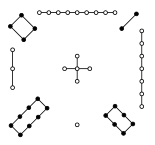
\includegraphics[scale=0.6]{img/luo-shu.png}}
 \subcaptionbox{Magic square of order 3}[0.45\linewidth]{
   \begin{tabular}{|c|c|c|}
   \hline
   4 & 9 & 2 \\
   \hline
   3 & 5 & 7 \\
   \hline
   8 & 1 & 6 \\
   \hline
   \end{tabular}
   \vspace{8mm}
 }
 \captionsetup{labelformat=empty}
 \caption{}
 \label{fig:luo-shu}
\end{figure}

This is known as Lo Shu Square, a magic square of order 3. The sum of the numbers in each row, column and diagonal is the same: 15. For example, the sum of the first row 4 + 9 + 2 = 15; and the sum of the third column 2 + 7 + 6 = 15; the sum of the diagonal from left up to right bottom 4 + 5 + 6 = 15. The insight to the carnival fifteen game is exactly the magic square. All three numbers sum to 15, form the rows, columns, and diagonals in that square. If the carnival man hold a secrete Lo Shu map, he is essentially playing the tick-tack-toe game with other people.

\begin{figure}[htbp]
 \centering
 \subcaptionbox{magic square}[0.45\linewidth]{
   \begin{tabular}{|c|c|c|}
   \hline
   4 & 9 & 2 \\
   \hline
   3 & 5 & 7 \\
   \hline
   8 & 1 & 6 \\
   \hline
   \end{tabular}
   \vspace{3mm}
 }
 \subcaptionbox{tick-tack-toe game}[0.45\linewidth]{
   \begin{tabular}{c|c|c}
   $\times$ &  & $\bigcirc$ \\
   \hline
   $\times$ & $\times$ &  \\
   \hline
   $\bigcirc$ & $\times$ & $\bigcirc$ \\
   \end{tabular}
   \vspace{3mm}
 }
 \captionsetup{labelformat=empty}
 \caption{}
 \label{fig:bingo-magic-square}
\end{figure}

The game between the lady and Mr. Carny is equivalent to such a tick-tack-toe game. The man trapped the lady in step three. He could line up both a column and a diagonal. If the lady puts on 3, then the man could win the game by playing on 5. If you know a bit about game theory or programming, one will never lose the tick-tack-toe game if plays carefully. The carnival man with the secrete Lo Shu square map does have the advantage over other people. As the fifteen game proceeds, the carnival operator mentally plays a corresponding tick-tack-toe game on his secrete map. This makes it easy for the operator to set up traps of winning position.

\begin{figure}[htbp]
 \centering
 \subcaptionbox{magic square}[0.45\linewidth]{
   \begin{tabular}{|c|c|c|}
   \hline
   4 & 9 & 2 \\
   \hline
   3 & 5 & 7 \\
   \hline
   8 & 1 & 6 \\
   \hline
   \end{tabular}
   \vspace{3mm}
 }
 \subcaptionbox{Step 1, the lady puts on 7, the man puts on 8.}[0.45\linewidth]{
   \begin{tabular}{c|c|c}
   &  & \\
   \hline
   &  & $\times$ \\
   \hline
   $\bigcirc$ & & \\
   \end{tabular}
   \vspace{3mm}
 } \vspace{3mm} \\
 \subcaptionbox{Step 2, the lady puts on 2, the man puts on 6.}[0.45\linewidth]{
   \begin{tabular}{c|c|c}
   &  & $\times$\\
   \hline
   &  & $\times$ \\
   \hline
   $\bigcirc$ & & $\bigcirc$ \\
   \end{tabular}
   \vspace{3mm}
 }
 \subcaptionbox{Step 3, the lady puts on 1, the man puts on 4.}[0.45\linewidth]{
   \begin{tabular}{c|c|c}
   $\bigcirc$ &  & $\times$\\
   \hline
   &  & $\times$ \\
   \hline
   $\bigcirc$ & $\times$ & $\bigcirc$ \\
   \end{tabular}
   \vspace{3mm}
 } \vspace{3mm} \\
 \subcaptionbox{Step 4, the lady puts on 5, the man wins on 3.}[0.45\linewidth]{
   \begin{tabular}{c|c|c}
   $\pmb{\bigcirc}$ &  & $\times$\\
   \hline
   $\pmb{\bigcirc}$ &  $\times$ & $\times$ \\
   \hline
   $\pmb{\bigcirc}$ & $\times$ & $\bigcirc$ \\
   \end{tabular}
   \vspace{3mm}
 }
 \captionsetup{labelformat=empty}
 \caption{}
 \label{fig:game-steps}
\end{figure}

This interesting story reflects an important mathematical idea, isomorphism. A difficult problem can be transformed to an isomorphic one, which is mathematical equivalent and easy to solve. A line of 9 numbers is isomorphic to a 3 x 3 grids; the sum target of fifteen is isomorphic to the rows, columns, and diagonals; Lo Shu pattern is isomorphic to magic square of order 3. This is what this book intents to tell: programming is isomorphic to mathematics. Just like in art and music, there are interesting stories and mathematicians behind the great minds.

There is another further idea in this story: under the surface of the problem hides the theoretical essence, which we need abstract and understand. With the rapid development of artificial intelligence and machine learning, can we keep moving forward with a little cleverness and engineering practice? Are we going to open the mysterious black box to find the map to the future?

\vspace{15mm}

Liu Xinyu

May 2019, Beijing

\begin{Exercise}
\Question{Implementing a tick-tack-toe game is a classic programming exercise. It's trivial to test if the sum of three numbers is 15. Please use this point to implement a simplified tick-tack-toe program that never lose game to human.}
\end{Exercise}

\vspace{10mm}

The book PDF can be downloaded from \url{https://github.com/liuxinyu95/unplugged}. Please contact with me through liuxinyu95@gmail.com if you want a hard copy.

\ifx\wholebook\relax \else

\expandafter\enddocument
%\end{document}

\fi
